\documentclass[10pt]{beamer}
% TODO: explain Electrum screenshots
% Bootstrap Icons https://icons.getbootstrap.com/
% svg2pdf https://github.com/typst/svg2pdf

\usetheme[progressbar=frametitle,numbering=none]{metropolis}
\usepackage{appendixnumberbeamer}

\usepackage{booktabs}
\usepackage{xfrac}

\usepackage{pgfplots}
\usepgfplotslibrary{dateplot}
\usetikzlibrary{calc}
\usepackage[absolute,overlay]{textpos} % for textblock* env

\usepackage{xspace}
\newcommand{\themename}{\textbf{\textsc{metropolis}}\xspace}

\title{Bitcoin: The Theoretical Minimum}
\subtitle{in-house seminar}
\date{2025-05-XX}
\author{Jeongho Jeon}
\institute{DSRV (All That Node, Custody, Payments, Validator, WELLDONE Studio)}
\titlegraphic{\hfill\includegraphics[height=3.0ex]{dsrv_logo_master_black}}

\begin{document}

\begin{textblock*}{3cm}(0.95\paperwidth,0.97\paperheight)
{\fontsize{2pt}{2.4pt}\selectfont\color{gray}version 20251029}
\end{textblock*}

\maketitle

\begin{frame}[fragile]{UTXO model}

Bitcoin and its forks use the UTXO model, while account-based
 models, like a bank balance, are easier to reason about.
 Account-based systems record balances in one place,
 making them better suited for smart contracts,
 as seen in Ethereum.

In the UTXO model, a user's coins are scattered across
 many outputs. Wallets sum them to show the total balance.
 Unlike the account-based model, UTXO allows parallel transfers,
 e.g., transfering coins from A, B and C to D, E and F
 in one transaction.
 Though harder to handle in smart contract engines,
 UTXO is well-suited for privacy coins.

A blockchain \emph{state} stores either UTXOs or account balances,
 depending on the model.
\end{frame}

\begin{frame}[fragile]{Bitcoin transaction}

\centering
\begin{tikzpicture}[transform shape, scale=1]

\tikzset{
  tx/.style={minimum width=3cm, minimum height=1cm, inner sep=0pt, fill=lightgray},
}

\clip (-5,-1.8) rectangle (5,1.8);
  
\node[tx,name=tx1] at (0,0) {};
  \node at ($(tx1)+(-1.3,0.17)$) {\includegraphics[width=0.25cm]{key.pdf}}; \node at ($(tx1)+(-0.9,0.17)$) {\tiny{input}};
  \node at ($(tx1)+(-1.3,-0.17)$) {\includegraphics[width=0.25cm]{key.pdf}}; \node at ($(tx1)+(-0.9,-0.17)$) {\tiny{input}};
  \node at ($(tx1)+(1.3,0.3)$) {\includegraphics[width=0.25cm]{lock.pdf}}; \node at ($(tx1)+(0.9,0.3)$) {\tiny{output}};
  \node at ($(tx1)+(1.3,0)$) {\includegraphics[width=0.25cm]{lock.pdf}}; \node at ($(tx1)+(0.9,0)$) {\tiny{output}};
  \node at ($(tx1)+(1.3,-0.3)$) {\includegraphics[width=0.25cm]{lock.pdf}}; \node at ($(tx1)+(0.9,-0.3)$) {\tiny{output}};
\node[tx,name=otx1] at (-5,0.9) {};
  \node at ($(otx1)+(1.3,0.3)$) {\includegraphics[width=0.25cm]{lock.pdf}};
  \node at ($(otx1)+(1.3,0)$) {\includegraphics[width=0.25cm]{lock.pdf}};
  \node at ($(otx1)+(1.3,-0.3)$) {\includegraphics[width=0.25cm]{lock.pdf}};
\node[tx,name=otx2] at (-5,-1.4) {};
  \node at ($(otx2)+(1.3,0.17)$) {\includegraphics[width=0.25cm]{lock.pdf}};
  \node at ($(otx2)+(1.3,-0.17)$) {\includegraphics[width=0.25cm]{lock.pdf}};
\node[tx,name=ntx1] at (5,0.6) {};
  \node at ($(ntx1)+(-1.3,0.3)$) {\includegraphics[width=0.25cm]{key.pdf}};
  \node at ($(ntx1)+(-1.3,0)$) {\includegraphics[width=0.25cm]{key.pdf}};
  \node at ($(ntx1)+(-1.3,-0.3)$) {\includegraphics[width=0.25cm]{key.pdf}};
\node[tx,name=ntx2] at (5,-1) {};
  \node at ($(ntx2)+(-1.3,0)$) {\includegraphics[width=0.25cm]{key.pdf}};

\draw[->,thick,draw=lightgray] ($(otx1.east)+(0.1,0.25)$) -- (0,6);
\draw[thick,draw=lightgray] ($(otx1.east)+(0.1,0)$) -- ($(otx1.east)+(0.3,0)$) node[right] {\tiny{UTXO}};
\draw[->,thick,draw=lightgray] ($(otx1.east)+(0.1,-0.25)$) -- ($(tx1.west)+(-0.1,0.17)$);

\draw[->,thick,draw=lightgray] ($(otx2.east)+(0.1,0.17)$) -- ($(tx1.west)+(-0.1,-0.17)$);
\draw[->,thick,draw=lightgray] ($(otx2.east)+(0.1,-0.17)$) -- (0,-5);

\draw[thick,draw=lightgray] ($(tx1.east)+(0.1,0.25)$) -- ($(tx1.east)+(0.3-0.1,0.25+0.5)$) node[above] {\tiny{UTXO}};
\draw[->,thick,draw=lightgray] ($(tx1.east)+(0.1,0)$) -- ($(ntx1.west)+(-0.1,-0.25)$);
\draw[->,thick,draw=lightgray] ($(tx1.east)+(0.1,-0.25)$) -- ($(ntx2.west)+(-0.1,0)$);

\draw[->,thick,draw=lightgray] (0,10) -- ($(ntx1.west)+(-0.1,0.25)$);
\draw[->,thick,draw=lightgray] (0,4) -- ($(ntx1.west)+(-0.1,0)$);

\end{tikzpicture}

\raggedright
A transaction consists of inputs and outputs.
 Think of it as melting old coins (inputs) and
 minting new ones (outputs). Each input references an
 \textbf{U}nspent \textbf{T}rans(\textbf{X})action \textbf{O}utput
 (UTXO) using the previous transaction hash and output index.

Outputs were locked with conditions,
 like a recipient address and related signature.
 Inputs provide the unlocking key, typically a digital signature.
 New outputs are created with new locks,
 defining who can spend the coins next.

\end{frame}

\begin{frame}[fragile]{no explicit fee}

\centering
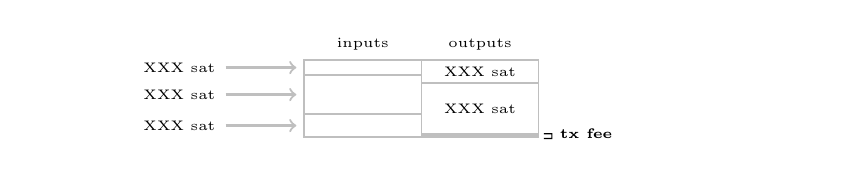
\begin{tikzpicture}[transform shape, scale=1]

\pgfmathsetlengthmacro{\width}{3cm}
\pgfmathsetlengthmacro{\height}{1cm}
\pgfmathsetlengthmacro{\shift}{0.02cm}
\pgfmathsetlengthmacro{\inputHeightA}{0.2cm-4*\shift/3}
\pgfmathsetlengthmacro{\inputHeightB}{0.5cm-4*\shift/3}
\pgfmathsetlengthmacro{\inputHeightC}{0.3cm-4*\shift/3}
\pgfmathsetlengthmacro{\outputHeightA}{0.3cm-3*\shift/2}
\pgfmathsetlengthmacro{\outputHeightB}{0.7cm-0.04cm-3*\shift/2}
\pgfmathsetlengthmacro{\partWidth}{(\width-3*\shift)/2}
\pgfmathsetlengthmacro{\xOffset}{\width/2-\shift-\partWidth/2}
\tikzset{
  tx/.style={minimum width=\width, minimum height=\height, inner sep=0pt, fill=lightgray},
  part/.style={minimum width=\partWidth, inner sep=0pt, fill=white},
}

\clip (-5,-0.6) rectangle (5,0.9);

\node[tx,name=tx1] at (0,0) {};
  % inputs
  \node[part, minimum height=\inputHeightA, name=input1] at ($(tx1)+(-\xOffset,\height/2-\shift-\inputHeightA/2)$) {};
  \node[part, minimum height=\inputHeightB, name=input2] at ($(tx1)+(-\xOffset,\height/2-\shift-\inputHeightA-\shift-\inputHeightB/2)$) {};
  \node[part, minimum height=\inputHeightC, name=input3] at ($(tx1)+(-\xOffset,-\height/2+\shift+\inputHeightC/2)$) {};
  % outputs
  \node[part, minimum height=\outputHeightA, name=output1] at ($(tx1)+(\xOffset,\height/2-\shift-\outputHeightA/2)$) {\tiny XXX sat};
  \node[part, minimum height=\outputHeightB, name=lastOutput] at ($(tx1)+(\xOffset,\height/2-\shift-\outputHeightA-\shift-\outputHeightB/2)$) {\tiny XXX sat};

\draw ($(lastOutput.south east) + (\shift,0) + (0.05,0)$) -- ++(0.1,0) -- ($(tx1.south east) + (0.15,0)$) -- ++(-0.1,0);
\node[anchor=west] at ($(lastOutput.south east) + (0.15,0)$) {\textbf{\tiny tx fee}};

\draw[->,thick,draw=lightgray] ($(input1.west)+(-1,0)$) node [anchor=east] {\tiny XXX sat} -- ($(input1.west)+(-0.1,0)$);
\draw[->,thick,draw=lightgray] ($(input2.west)+(-1,0)$) node [anchor=east] {\tiny XXX sat} -- ($(input2.west)+(-0.1,0)$);
\draw[->,thick,draw=lightgray] ($(input3.west)+(-1,0)$) node [anchor=east] {\tiny XXX sat} -- ($(input3.west)+(-0.1,0)$);

\node[anchor=south] at (input1.north) {\tiny inputs};
\node[anchor=south] at (output1.north) {\tiny outputs};

\end{tikzpicture}

\raggedright
Bitcoin transactions don't explicitly show the fee.
 The fee is calculated as total input amount minus total output amount.
 Miners collect the fee as a reward.
 While outputs show coin amounts,
 input values must be traced back to previous transactions.

Bitcoin fees are measured in sat/vB (satoshis per virtual byte,
 see SegWit for `virtual').
 Miners collect transactions into 1 MB blocks and
 prefer txs with higher fees per byte.
 Fees are not based on the coin amount, but on transaction size.
 Transaction size increases with more inputs and outputs.

Coins that cost more to spend than they're worth are called \emph{dust}.
 Wallet developers avoid selecting inputs that would leave dust.
 SDKs don't handle this automatically.
\end{frame}

\begin{frame}[fragile]{change}

It's rare for inputs to exactly match outputs plus fees.
 The leftover amount output is sent back to the sender as \emph{change}.

Bitcoin recommends changing addresses with each use.
 Unlike MetaMask, which shows one address at a time,
 Bitcoin wallets often display 20+ addresses.
 These addresses are derived from the same mnemonic,
 but appear unrelated to outsiders.

\end{frame}

\begin{frame}[fragile]{transaction fee bumping}

Two common strategies exist to handle transactions waiting
 in the mempool, often due to low fees.
 
\begin{description}
\item[Replace By Fee (RBF)]
  A transaction with an input's ``sequence'' field below
  \texttt{0xfffffffe} is replaceable. To replace a transaction,
  create a new one that spends at least one of the same UTXOs
  with a higher fee.
  Fees can be increased by including more inputs or
  lowering output values.
\item[Child Pays for Parent (CPFP)]
  Without replacing the original transaction, you can attach a
  high-fee child transaction that spends its output.
  To claim the higher fee, miners are incentivized to include
  the low-fee parent transaction along with the high-fee child
  one in the same block. Even recipients can use this method
  to accelerate confirmation.
\end{description}

\end{frame}

\begin{frame}[fragile]{coinbase transaction}

Bitcoin transactions can have any number of inputs and outputs.
 For example, a mining pool reward distribution transaction may
 have 1 input and over 100 outputs.

Some special transactions create new bitcoins without spending any inputs.
 These are \emph{coinbase transactions}, which reward miners.
 Each block starts with a coinbase transaction.
 It has one dummy input that isn't interpreted.
 It is typically used for extranonce and mining pool names.
 Satoshi's famous message,
 \textit{The Times 03/Jan/2009 \ldots\ bailout for banks.}, was here.

The coinbase transaction's output amount equals the block reward
 plus the total fees from all transactions in the block.
 SegWit introduced an additional zero-valued output
 carrying the wtxid (txid with witness) Merkle tree root.

\end{frame}

\begin{frame}[fragile]{Bitcoin script}

To spend a UTXO, \includegraphics[height=1em]{key.pdf} (scriptSig)
 + \includegraphics[height=1em]{lock.pdf} (scriptPubKey) are
 executed in order. If the result is true, the spend is allowed.
 Let's take a legacy P2PKH (Pay to Public Key Hash) transaction
 as an example.

{\scriptsize \includegraphics[height=1em]{key.pdf} (new tx's input) -
 <sig> <pubKey> \\
\vspace{-0.5\baselineskip}\includegraphics[height=1em]{lock.pdf}
 (old tx's output) - \texttt{OP\_DUP} \texttt{OP\_HASH160}
 <pubKeyHash> \texttt{OP\_EQUALVERIFY} \texttt{OP\_CHECKSIG}}

As commands are executed in order, the stack looks like this:

\scriptsize
\begin{tabular}{r|l}
\toprule
command & stack \\
\midrule
<sig> & \colorbox{green!20}{<sig>} \\
<pubKey> & <sig> \colorbox{green!20}{<pubKey>} \\
\texttt{OP\_DUP} (duplicate the last) & <sig> <pubKey> \colorbox{green!20}{<pubKey>} \\
\texttt{OP\_HASH160} (hash the last) & <sig> <pubKey> \colorbox{green!20}{<pubKeyHash>} \\
<pubKeyHash> & <sig> <pubKey> <pubKeyHash> \colorbox{green!20}{<pubKeyHash>} \\
\texttt{OP\_EQUALVERIFY} (fail if not equal) & <sig> <pubKey> \\
\texttt{OP\_CHECKSIG} (check the last's signature) & \colorbox{green!20}{true} \\
\bottomrule
\end{tabular}

\normalsize
With an invalid signature, the script fails and the UTXO cannot be spent.

\end{frame}

\begin{frame}[fragile]{standard transaction types}

Most nodes only relay and mine standard transaction types.
 Transactions that create dust may be rejected or not mined.
 In addition to P2PKH, standard Bitcoin transaction types include:

\begin{description}
\item[P2PH (Pay to Public Key)]
 This output exposed the public key and was used briefly in the early days. \\
{\scriptsize
 \vspace{0.2\baselineskip}\includegraphics[height=1em]{key.pdf}
 (new tx's input) - <sig> \\
\vspace{-0.5\baselineskip}\includegraphics[height=1em]{lock.pdf}
 (old tx's output) - <pubKey> \texttt{OP\_CHECKSIG}}

\item[\texttt{OP\_RETURN}]
  \texttt{OP\_RETURN} creates an unspendable output.
  It can store arbitrary data on Bitcoin,
  which Bitcoin does not interpret.
  This enabled overlay protocols like Colored Coins and Mastercoin.
  Some believe these were early forms of NFT.
  Since it's unspendable, it has no amount. \\
{\scriptsize
 \vspace{0.2\baselineskip}\includegraphics[height=1em]{key.pdf}
 (new tx's input) - \textcolor{red!70}{unspendable} \\
\vspace{-0.5\baselineskip}\includegraphics[height=1em]{lock.pdf}
 (old tx's output) - \texttt{OP\_RETURN} <arbitrary data>}
\end{description}

\end{frame}

\begin{frame}[fragile]{standard transaction types}

\begin{description}
\item[P2SH (Pay to Script Hash)] 
  With \texttt{OP\_IF} and \texttt{OP\_ELSE}, complex conditions
  can be written, for example, requiring 2-of-3 guardian signatures
  until the heir becomes an adult.
  But this increases output size and UTXO set. To address this,
  P2SH was introduced: only a script hash is stored in the output,
  and the full script is revealed when spending. \\
{\scriptsize
 \vspace{0.2\baselineskip}\includegraphics[height=1em]{key.pdf}
 (new tx's input) - \texttt{OP\_HASH160} <scriptHash>
 \texttt{OP\_EQUAL} \\
\vspace{-0.5\baselineskip}\includegraphics[height=1em]{lock.pdf}
 (old tx's output) - <param$_1$> \ldots <param$_N$> <script>}

\vspace{0.2\baselineskip}The script may use \texttt{OP\_CHECKMULTISIG}
 to require multiple signatures for spending.
 Taproot replaces this with more efficient \texttt{OP\_CHECKSIGADD}. \\
{\scriptsize
 \vspace{0.2\baselineskip}\includegraphics[height=1em]{key.pdf}
 (new tx's input) - 0\textcolor{gray!70}{(dummy)} <sig$_1$> <sig$_2$> \\
\vspace{-0.5\baselineskip}\includegraphics[height=1em]{lock.pdf}
 (old tx's output) - 2 <pubKey$_1$> <pubKey$_2$> <pubKey$_3$> 3
 \texttt{OP\_CHECKMULTISIG}} \\
{\scriptsize
 \vspace{0.4\baselineskip}\includegraphics[height=1em]{key.pdf}
 (new tx's input) - <sig$_3$> dummy <sig$_1$> \\
\includegraphics[height=1em]{lock.pdf}
 (old tx's output) - <pubKey$_1$> \texttt{OP\_CHEKCSIG} <pubKey$_2$>
 \texttt{OP\_CHEKCSIGADD} \\
\vspace{-0.5\baselineskip}\hspace{8em}<pubKey$_3$>
 \texttt{OP\_CHEKCSIGADD} 2 \texttt{OP\_GREATERTHANOREQUAL}}
\end{description}

\end{frame}

\begin{frame}[fragile]{SegWit (Segregated Witness)}

SegWit soft fork was introduced in 2017 after the blocksize war.
 It moved bulky signatures to a new ``witness''
 section, counted at $\sfrac{1}{4}$ bytes.
 This allowed more transactions per 1MB block, reduced fees, and led to the concept of vbytes: 1 vbyte = 4 weight.

If a node assumes transactions were already validated by others,
 it doesn't need the witness to understand its effects.
 This allows for lighter relaying and storage.

Also, since random signatures no longer affect the txid (tx hash),
 the malleability issue is resolved, enabling dependency-sensitive
 L2 solutions like Lightning Network.

Finally, SegWit made it easier to introduce new features
 through version upgrades.

\end{frame}

\begin{frame}[fragile]{SegWit (Segregated Witness)}

SegWit introduced P2WPKH and P2WSH---the SegWit versions of
 P2PKH and P2SH. A P2WPKH script looks like this: \\
{\scriptsize
 \vspace{0.2\baselineskip}\includegraphics[height=1em]{key.pdf}
 (new tx's input) - empty (<sig> <pubKey> in witness) \\
\vspace{-0.5\baselineskip}\includegraphics[height=1em]{lock.pdf}
 (old tx's output) - 0\textcolor{gray!70}{(version)} <pubKeyHash>}

SegWit uses lowercase Bech32 addresses (same as Cosmos) that
 start with `bc1', visually distinct from legacy mixed-case
 Base58Check addresses that start with `1' or `3'.

\end{frame}

\begin{frame}[fragile]{Taproot}

Taproot soft fork (2021) introduced support for easily
 aggregatable Schnorr signatures.
 It uses SegWit version 1 and Bech32m addresses.
 Spend conditions are organized in a Merkle tree,
 revealing only the script used---improving block space and privacy.
 P2TR (Pay to Taproot) outputs can be spent in one of two ways.

{\scriptsize \includegraphics[height=1em]{lock.pdf}
 (old tx's output) - 1\textcolor{gray!70}{(version)} <taprootAddress>}
 
\begin{description}
\item[key path spending] with one aggregated signature
  (implying consent from all parties) \\
  {\scriptsize
  \vspace{0.2\baselineskip}\includegraphics[height=1em]{key.pdf}
  (new tx's input) - empty (<sig> in witness)}
\item[script path spending] with the satisfying script
  and its Merkle proof. Check if a Taproot address $Q$ can be
  created from The Merkle tree root $m$ calculated from
  the Merkle proof. \\
  $Q = P + hash(P \Vert m) \cdot G$ \\
  {\scriptsize
  \vspace{0.2\baselineskip}\includegraphics[height=1em]{key.pdf}
  (new tx's input) - empty (<param$_1$> \ldots <script> <controlBlock>
  in witness) \\
  \vspace{-0.5\baselineskip}<controlBlock> contains
  internal public key $P$ and Merkle proof.}
\end{description}

\end{frame}

\begin{frame}[fragile]{Taproot}

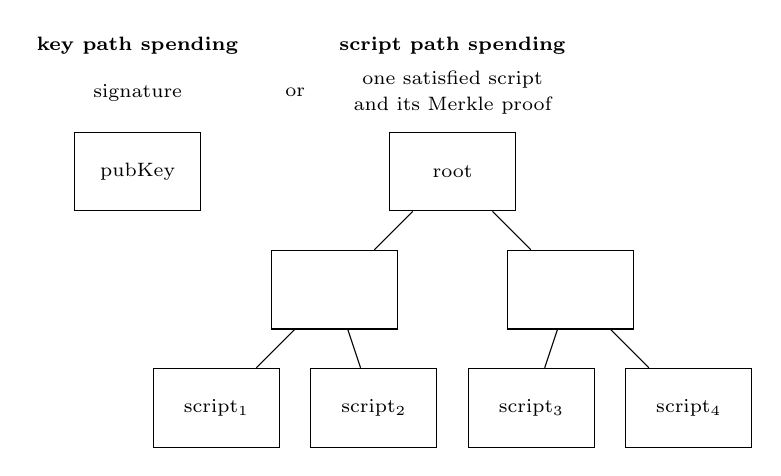
\begin{tikzpicture}[transform shape, scale=1]

\tikzset{
  box/.style={minimum width=1.6cm, minimum height=1cm, inner sep=0pt, draw},
  boxedg/.style={},
}

\node at (-4,1.6) {\scriptsize \textbf{key path spending}};
\node at (0,1.6) {\scriptsize \textbf{script path spending}};
\node at (-4,1) {\scriptsize signature};
\node at (-2,1) {\scriptsize or};
\node[align=center] at (0,1) {\shortstack{\scriptsize one satisfied script \\ \scriptsize and its Merkle proof}};
\node[box,name=pubKey] at (-4,0) {\scriptsize pubKey};
\node[box,name=root] at (0,0) {\scriptsize root};
\node[box,name=nd11] at (-1.5,-1.5) {};
\node[box,name=nd12] at (1.5,-1.5) {};
\node[box,name=nd21] at (-3,-3) {\scriptsize script$_1$};
\node[box,name=nd22] at (-1,-3) {\scriptsize script$_2$};
\node[box,name=nd23] at (1,-3) {\scriptsize script$_3$};
\node[box,name=nd24] at (3,-3) {\scriptsize script$_4$};

\draw[boxedg] (root) -- (nd11);
\draw[boxedg] (root) -- (nd12);
\draw[boxedg] (nd11) -- (nd21);
\draw[boxedg] (nd11) -- (nd22);
\draw[boxedg] (nd12) -- (nd23);
\draw[boxedg] (nd12) -- (nd24);

\end{tikzpicture}

\end{frame}

\begin{frame}[fragile]{Babylon}

Bitcoin uses PoW and has no native staking.
 However, ideas emerged to earn yield on idle BTC---Babylon is
 one example.
 Unlike typical protocols that lock tokens like bridges,
 Babylon promotes self-custodial staking and on-demand unbonding.

Most staking operations, including rewards, happen on the
 Babylon chain (Cosmos SDK + Cosmwasm engine).
 There are daemon programs monitor Babylon Bitcoin staking transactions.

Babylon uses Taproot transactions on the Bitcoin chain.
 Since a public key that no one knows the private key for is used,
 key path spending is not possible, and only script path spending
 is allowed.

\end{frame}

\begin{frame}[fragile]{Babylon}

The script requires signatures from the staker (user),
 finality provider (validator), and covenant committee
 (which is selected by governance and requires a quorum
 of 6 out of 9 members).
When creating a staking transaction, the staker must pre-sign
 unbonding transaction and slashing transaction in advance.

Three scripts are used in Taproot transactions:

\begin{description}
\item[Timelock path] after the staking period ends \\
  {\scriptsize <stakerPubKey> OP\_CHECKSIGVERIFY <timelockInBlocks> OP\_CSV}
\item[Unbonding path] withdrawal during the staking period \\
  {\scriptsize \vspace{0.2\baselineskip}<stakerPubKey> OP\_CHECKSIGVERIFY \\
  \vspace{-0.5\baselineskip}<covenantPubKey$_1$> OP\_CHECKSIG \ldots\ OP\_CHECKSIGADD <n> OP\_NUMEQUAL}
\item[Slashing path] upon a slashing event.
  When double signing occurs, the finality provider private key
  is revealed, allowing anyone to generate an finality provider
  signature. \\
  {\scriptsize \vspace{0.2\baselineskip}<stakerPubKey> OP\_CHECKSIGVERIFY \\
  <finalityProviderPubKey> OP\_CHECKSIGVERIFY \\
  \vspace{-0.5\baselineskip}<covenantPubKey$_1$> OP\_CHECKSIG \ldots\ OP\_CHECKSIGADD <n> OP\_NUMEQUAL}
\end{description}

\end{frame}

\begin{frame}[fragile]{Babylon Bitcoin transactions}

\centering
\begin{tikzpicture}[transform shape, scale=1]

\tikzset{
  tx/.style={minimum width=1.6cm, minimum height=1cm, inner sep=0pt, fill=lightgray},
  edg/.style={->, thick, rounded corners=20pt, dashed, dash pattern=on 4pt off 2pt, line width=3pt, color=lightgray},
  edglbl/.style={font=\tiny,color=black},
}
  
\node[tx,name=stakingTx] at (-3,0) {\scriptsize staking tx};
\node[tx,name=withdrawalTx] at (3,2) {\scriptsize withdrawal tx};
\node[tx,name=unbondingTx] at (0,0) {\scriptsize unbonding tx};
\node[tx,name=slashingTx] at (3,-2) {\scriptsize slashing tx};

\draw[edg,solid] ($(stakingTx.west)+(-1,0)$) -- node[edglbl,pos=0.2,yshift=-1.5em,align=center] {any funding \\ inputs} ($(stakingTx.west)+(-0.1,0)$);
\draw[edg] 
  ($(stakingTx.east)+(0.1,0.25)$) --
  ($(stakingTx.east)+(0.5,0.25)$) |- ($(withdrawalTx.west)+(-0.1,0)$) node[edglbl,pos=0.6,above] {case 1: Timelock path};
\draw[edg] 
  ($(stakingTx.east)+(0.1,0.25)$) -- ($(unbondingTx.west)+(-0.1,0.25)$) node[edglbl,midway,above,yshift=0.8em,xshift=2.8em] {case 2: Unbonding path};
\draw[edg] 
  ($(stakingTx.east)+(0.1,0.25)$) --
  ($(stakingTx.east)+(0.5,0.25)$) |- ($(slashingTx.west)+(-0.1,0)$) node[edglbl,pos=0.6,yshift=-1em] {case 3: Slashing path};
\draw[edg] 
  ($(unbondingTx.east)+(0.1,0.25)$) --
  ($(unbondingTx.east)+(0.5,0.25)$) |- ($(withdrawalTx.west)+(-0.1,0)$) node[edglbl,pos=0.3,right] {case 2--1: Timelock path};
\draw[edg] 
  ($(unbondingTx.east)+(0.1,0.25)$) --
  ($(unbondingTx.east)+(0.5,-0.25)$) |- ($(slashingTx.west)+(-0.1,0)$) node[edglbl,pos=0.3,right] {case 2--2: Slashing path};
\draw[edg,solid] 
  ($(stakingTx.east)+(0.1,-0.25)$) -- ($(stakingTx.east)+(1.0,-0.25)$) node[edglbl,midway,below,yshift=-0.8em,xshift=-2.4em] {\shortstack{\tiny OP\_RETURN metadata \\ \tiny (includes staker public key, \\ \tiny finality provider public key \\ \tiny and staking period)}};

\draw[edg,solid] 
  ($(unbondingTx.east)+(0.1,-0.25)$) -- ($(unbondingTx.east)+(1.0,-0.25)$) node[edglbl,yshift=0em,xshift=4em] {output that burns unbonding fee}

\draw[edg,solid] 
  ($(withdrawalTx.east)+(0.1,0.0)$) -- ($(withdrawalTx.east)+(1.0,0.0)$) node[edglbl,midway,below,yshift=-0.2em,xshift=1.2em] {\shortstack{\tiny freely spendable \\ \tiny output}}

\draw[edg,solid] 
  ($(slashingTx.east)+(0.1,0.25)$) -- ($(slashingTx.east)+(1.0,0.25)$) node[edglbl,midway,above,yshift=0.2em,xshift=1.2em] {timelock output}
\draw[edg,solid] 
  ($(slashingTx.east)+(0.1,-0.25)$) -- ($(slashingTx.east)+(1.0,-0.25)$) node[edglbl,midway,below,yshift=-0.2em,xshift=1.2em] {\shortstack{\tiny output that \\ \tiny burns slashing}}

%\node[anchor=west] at ($(slashingTx.east)+(0,0.3)$) {\shortstack{\scriptsize timelock output}};
%\node[anchor=west] at ($(slashingTx.east)+(0,-0.4)$) {\shortstack{\scriptsize output that \\ \scriptsize burns slashing}}; 

\begin{scope}[shift={(-2.2,1.2)},scale=0.15]
\tikzset{
  box/.style={minimum width=1.6cm, minimum height=1cm, inner sep=0pt, draw,font=\huge\bfseries},
  boxedg/.style={},
}
\node[box,name=root] at (0,0) {};
\node[box,name=nd11] at (-1.5,-1.5) {};
\node[box,name=nd12] at (1.5,-1.5) {3};
\node[box,name=nd21] at (-3,-3) {1};
\node[box,name=nd22] at (-1,-3) {2};

\draw[boxedg] (root) -- (nd11);
\draw[boxedg] (root) -- (nd12);
\draw[boxedg] (nd11) -- (nd21);
\draw[boxedg] (nd11) -- (nd22);
\end{scope}

\begin{scope}[shift={(1.8,0.7)},scale=0.15]
\tikzset{
  box/.style={minimum width=1.6cm, minimum height=1cm, inner sep=0pt, draw,font=\huge\bfseries},
  boxedg/.style={},
}
\node[box,name=root] at (0,0) {};
\node[box,name=nd11] at (-1.5,-1.5) {2--1};
\node[box,name=nd12] at (1.5,-1.5) {2--2};

\draw[boxedg] (root) -- (nd11);
\draw[boxedg] (root) -- (nd12);
\end{scope}

\end{tikzpicture}

\end{frame}

\begin{frame}[fragile]{topics not covered}

\begin{itemize}
\item atomic swap and Lightning Network
\item soft fork activation
\item Inscriptions NFT
\item selfish mining
\item script hash types
\item \ldots
\end{itemize}

\end{frame}

\end{document}
